%!TEX root = ../thesis.tex
\chapter{Extraction of 3D Anatomical Structure}
\dblspace

\section{Aims} % (fold)
\label{sec:aims}
  
% section aims (end)

\section{Methods} % (fold)
\label{sec:methods}
  We can construct a matrix $S_0$ from the Cartesian product of the gradient of an image $I$. For illustrative purposes, let us consider a 2-dimensional image $I(x,y)$, so that
  
  \begin{align}
    S_0 &= \nabla I^T \, \nabla I \\
        &= \begin{pmatrix}
      I_x \\
      I_y
    \end{pmatrix} \begin{pmatrix}
      I_x && I_y
    \end{pmatrix} \\
        &= \begin{pmatrix}
          I_x^2 && I_xI_y \\
          I_xI_y && I_y^2
        \end{pmatrix}.
  \end{align}
  
  Because of the associativity of matrix multiplication, we can see that a multiplication of a vector $v$ with any matrix constructed from the Cartesian product of a vector $u$ will simply result in a vector parallel to $u$, with magnitude equal to the dot product of $v$ and $u$ multiplied by the magnitude of $u$. In our case,
  
  \begin{align}
    S_0 \mathbf{v} &= (\nabla I^T \, \nabla I) \mathbf{v} \\
                   &= (\nabla I \cdot \mathbf{v}) \nabla I^T.
  \end{align}
  
  From this it is clear that $S_0$ is a tensor with two eigenvectors, parallel with and perpendicular to $\nabla I$, with eigenvalues of $|\nabla I|^2$ and 0, respectively.
  
  The structure tensor $S_w$ is a matrix derived from this Cartesian product of the gradient of an image, which gives a measure of the magnitude and coherence of changes in intensity across a small image region. It is defined as the weighted mean of $S_0$ within a surrounding window $w$ of a given point in $I$. Equivalently, it is the convolution of $S_0$ with the windowing function.
  
  If the gradients are all coherently aligned well within a window, the largest eigenvector of the resulting $S_w$ will be much greater than the other eigenectors, and in 3-D, the tensor will take a long, thin shape. Clearly, $S_0$ is itself perfectly coherent. Gradients may also be distributed throughout a subspace of the entire space; in 3-D, gradients varying evenly within a 2-D plane will result in a flat, disc-shaped tensor, with one small eigenvalue associated with a vector perpendicular to that plane. If gradients are more isotropic, then all eigenvalues will be of a similar magnitude, giving a spherical tensor, and a zero tensor can only obtained if the gradient is zero throughout the windowing region.
  
  In a perfectly registered histological volume, and at the scale of individual myocardial cells, the smallest intensity gradients will be found parallel to the fibre direction, and the largest in the plane perpendicular to them. The structure tensors should therefore appear disc-shaped, with their short axis aligned with the muscle fibres.
  
  We apply the structure tensor to the regionally registered block from Section~\ref{sub:regional_diffusion}. It is important to have the same sampling rate within the plane of the slices as between them, so that artificial anisotropy is not introduced. A volume is therefore constructed from slice images that are downsampled and Gaussian smoothed so as to have the same spatial resolution of 10$\mu$m as the slicing.
% section methods (end)

\section{Results} % (fold)
\label{sec:results}
  \begin{sidewaysfigure}[htbp]
    \centering
    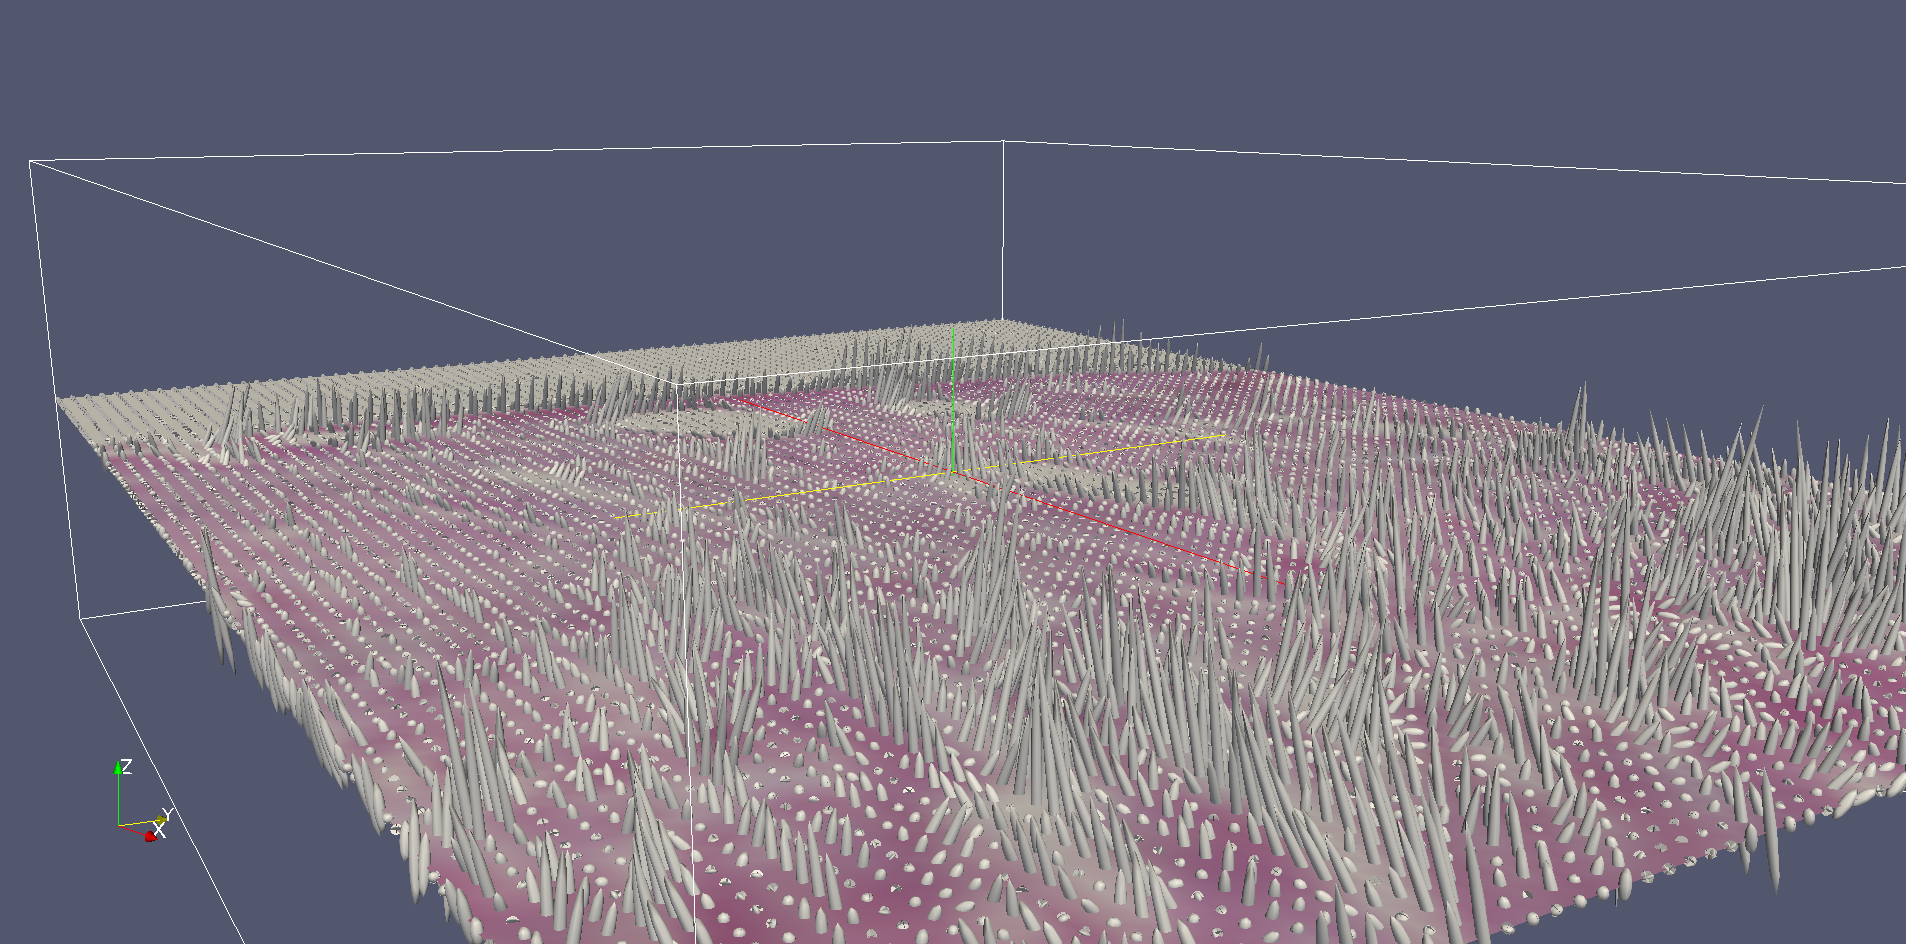
\includegraphics[width=\textwidth]{Ch8/Figs/structure_tensor_glyphs}
    \caption{A central slice through the epicardial vessel region from Section~\ref{sub:regional_diffusion}, overlayed with spheroid glyphs, scaled and oriented by the structure tensor of the pixel intensities.}
    \label{fig:structure_tensor_glyphs}
  \end{sidewaysfigure}
    
  \begin{figure}[htbp]
    \centering
    \subfigure[][x]{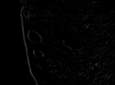
\includegraphics[width=0.45\textwidth]{Ch8/Figs/x_eigencomponent.png}}
    \subfigure[][y]{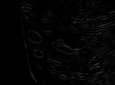
\includegraphics[width=0.45\textwidth]{Ch8/Figs/y_eigencomponent.png}}
    \subfigure[][z]{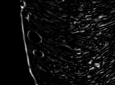
\includegraphics[width=0.45\textwidth]{Ch8/Figs/z_eigencomponent.png}}
    \subfigure[][combined]{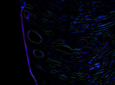
\includegraphics[width=0.45\textwidth]{Ch8/Figs/rgb_eigencomponents.png}}
    \caption{\textbf{(a)}, \textbf{(b)} and \textbf{(c)} map the absolute magnitudes of the x-, y- and z- components of the largest eigenvector of the structure tensor, of the same central slice from Figure~\ref{fig:structure_tensor_glyphs}. The volumewise maximums for the x-, y-, and z- components were 15.8, 14.6 and 68.7, respectively; the intensities have thus been scaled from 0 (black) to 68.7 (white). \textbf{(d)} combines the intensities in an RGB image, with red x, green y and blue z.}
    \label{fig:eigencomponents}
  \end{figure}
  
% section results (end)

\section{Discussion} % (fold)
\label{sec:discussion}
  
% section discussion (end)
